%!TEX root = ../Thesis.tex
\chapter{Synopsis}
\label{sec:synopsis}
The following chapters are comprised of four journal papers that are supplemented with two conference papers and four workshop papers, of which all are peer-reviewed or submitted to peer-reviewed journals. I combine several papers into topical chapters for conciseness. This thesis follows a data science workflow, starting with exploratory data analysis to gain insight to the specific geology and 4D seismic. I go on to present groundwork on machine learning and data processing on 4D seismic data of the Danish North Sea. Based on this groundwork, I developed a method for 4D seismic inversion and a novel unsupervised 3D time-shift extraction method for 4D seismic. This chapter summarizes these papers and places them in the appropriate context for the thesis.

%!TEX root = ../Thesis.tex
\section{Data Preparation}
% aabo2017correlation
% aabo2018integrated
% dramsch2018gaussian

In \cref{sec:dataprep} I include one published journal paper \citep{aabo2018integrated}, one published conference paper \citep{aabo2017correlation}, and one published workshop paper \citep{dramsch2018gaussian}. The published conference paper with the title \citetitle{aabo2017correlation} \citep{aabo2017correlation} contains preliminary work contributing to and extended in the journal paper \citetitle{aabo2018integrated} \citep{aabo2018integrated}. Whereas, the workshop paper with the title \citetitle{dramsch2018gaussian} \citep{dramsch2018gaussian} is an independent study of backscatter scanning-electron microscopy data on chalk thin slices.

The data for this thesis was acquired in the Danish North Sea. The main hydrocarbon reservoirs in the Danish Central Graben area consist of chalk, a sedimentologically distinct feature in the seismic data. The chalk layer is high in porosity (20-35\%), however, very low in permeability 3~mD to less than 1~mD. In \citet{aabo2017correlation} we presented an integrated fracture study of the Ekofisk chalk Kraka field in the South Central Graben. Within this preliminary study, we performed a localized fracture study along one well-bore to compare fracture measurements from core, well logs and seismic data. Initial analysis of the seismic data showed a maximum vertical resolution of \textasciitilde40~m, which did not yield sufficient results for comparative study. 
% These data were prepared individually by three researchers, with my contribution being the analysis and preparation of the seismic dataset. 

\begin{figure}[!ht]
    \centering
    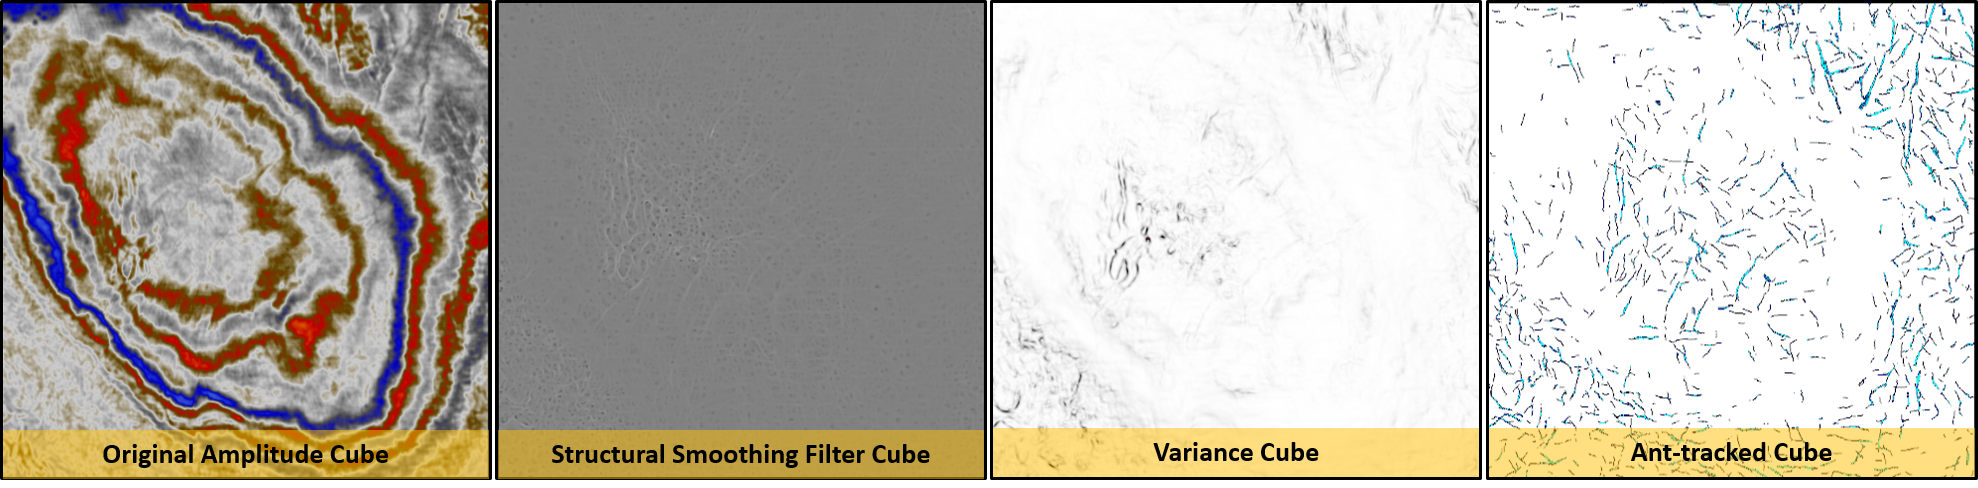
\includegraphics[width=\textwidth]{figures/seismic-comparisons.png}
    \caption{Comparison of seismic data, variance, and ant-track time slice to enhance fractures in images \citep[modified from][]{aabo2018integrated}}
    \label{fig:seismic-comparison}
\end{figure}

\cref{fig:seismic-comparison} contains several post-stack seismic attributes to enhance lineaments within the seismic cubes. While the variance and structural cubes yielded some initial promise the following image processing workflow yielded the best results. These were geared towards enhancing vertically coherent structures. This was achieved by a workflow including colorspace transformations and ant-tracking, which is a search algorithm leveraging biologically inspired software agents.

Normally, images are shown in \ac{rgb} colorspace, however, these can be transformed into other space, such as, \ac{cmyk} and \ac{hsv}. The \ac{hsv} colorspace is commonly used in image analysis to detect edges on the gradient of the saturation values. Therefore, it serves as a good target colorspace for image processing. To achieve this, the bit-depth of post-stack seismic data (8 / 16 bit) has to be increased, considering that natural images displayed on modern monitors contain \~32 million colors with a bit-depth of 24~bit for color representation.
This is achieved by replicating the seismic cubes with a static timeshift to create an \ac{rgb} representation \citep{laake2014structural}. In our case a small shift below 3~ms to avoid loss of small-scale fractures and avoid smearing yielded the best results. 

Consequently, after a colorspace transformation to \ac{hsv}, the biologically inspired ant-track algorithm was applied to the saturation gradient volume. The ant-tracking algorithm implements unsupervised software-agents that search the vicinity in a 3D volume to find spatially coherent features \citep{dorigo1992optimization}. The software agents can be instructed to be more or less aggressive in their search, which provides a trade-off between better fault vertical enhancement or nuance of the smaller fractures. The workflow for fault extraction is shown in \cref{fig:seismic-workflow}.

\begin{figure}[!ht]
    \centering
    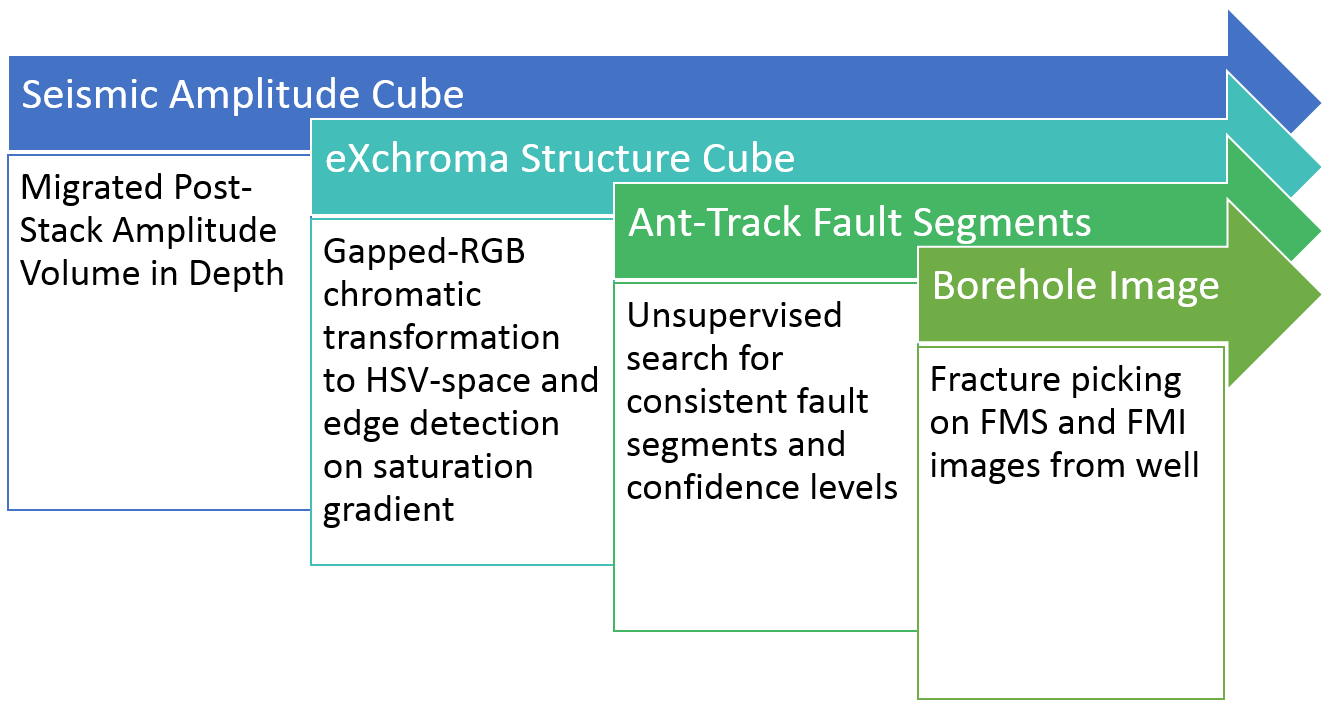
\includegraphics[width=\textwidth]{figures/fracture-workflow.PNG}
    \caption{Workflow to identify fractures in post-stack seismic data to prepare for comparison to \ac{bhi} analysis}
    \label{fig:seismic-workflow}
\end{figure}

Joint interpretation of the seismic and ant-track volumes yielded a focused seismic interpretation along the well-bore, where \acf{bhi} data were available for comparison (after the interpretation to avoid bias). These match the independent interpretation of the well data closely in orientation and distribution of fractures. It is likely that these represent fracture corridors, small faults or damage zones in the chalk. This preliminary study was able to show that seismic provides a valuable method for mapping the size, orientation and connectivity of fracture zones away from the well. 

Following this initial study, the seismic interpretation was extended for to regional fault systems and \ac{bhi} to several wells for \citet{aabo2018integrated} presented in \cref{sec:tala}. The analysis of ant-tracked attribute volumes, allowed us to relate structural trends below the resolution of amplitude seismic to features at different scales. This interpretation suggests that the fracture pattern is more complex than previously suggested. We propose that fracture generation and propagation in the field is in part controlled by the regional maximum horizontal stress from the seismic interpretation in addition to the halokinesis in the South Central Graben. 

The seismic analysis was correlated with the fracture analysis from \ac{bhi} data and core analysis in multiple wells. The fracture analysis was particularly dependent on the Terzaghi-correction \citep{terzaghi1965sources} to obtain the in-situ fracture orientation. This work identified two main fracture trends in the Danian Ekofisk reservoir. The main fracture set strikes sub-parallel to the regional NE/NNE maximum horizontal stress present on all horizontal/deviated wellbores and core. The vertical fracture distribution of the Kraka Field studied in a single well, due to availability. Within this single well the NE/NNE fracture distribution was continuous. This main NNE/NE fracture trend was traced from well scale to ant-tracked scale bridgeing the scale-gap. Regional large-scale faults interpreted on the raw amplitude seismic are present in the ant-tracked cube, trending NE, which indicates that the NNE trend is representative for smaller-scale lineations, with a Northern deviation on regional scales. 

Further research into the porosity and sedimentology of the chalk reservoirs conducted on microscoping scales focused on identifying porosity using \acf{bsem} in \cref{section:gaussian}, which comprises the third paper in this chapter \citep{dramsch2018gaussian}. Identifying the grain size and orientation of the oolites is usually a manual work-intensive task, ideal for computer vision tasks, considering the good contrast of light-grey to white oolites and the black background. Unfortunately, training data was not available, so unsupervised clustering was appropriate to find the optimal boundary of the grains. Gaussian Mixture Models learnt a two-fold representation that separated the background well from the rock. Any single-valued decision boundary will be non-smooth, which can be alleviated by morphological filtering. Smooth boundaries are essential for chalk grains, as the perimeter of the oolites can be used to calculate the specific surface of chalk. The optimal boundary of chalk grains could then be used to generate training data for more sophisticated machine learning systems.

% This chapter enabled me to explore the Danish North Sea data in Kraka, Dan and Halfdan, as well as, implement data science principles on geological problems. Collaborating with geologists on these papers resulted in a better understanding of underlying processes in the chalk and 4D effects of production, due to compaction, stimulation and chalk weakening. The seismic analysis improved my understanding of the geological structures and trendlines in the South Central Graben area, while contributing to an improved understand of the scale-dependence of the stress fields and a method capable of extracting an optimal boundary of chalk in \ac{bsem}. 

In the first study of this chapter \citep{aabo2017correlation} we applied an image processing workflow to enhance the vertical resolution of seismic data. Consequently, The data was transformed to deploy a biologically inspired software algorithm to enhance and identify lineaments for better interpretation. This work was essential in enabling a localized pilot study to relate localized features from well-scale \ac{bhi} to enhanced seismic-scale, verifying the seismic image analysis. This pilot study fed into a larger study \citep{aabo2018integrated}, where a fracture study from core and \ac{bhi} was related to both the enhanced ant-tracked volume and a regional fault interpretation, updating the understanding of the fracture generation in the Salt Dome Process in the Danish South Central Graben area. The third study solved a manual process using an unsupervised image analysis tool paired with strong data science principles, providing a novel reliable tool to geologists in \ac{bsem} analysis.

%!TEX root = ../Thesis.tex
\section{Foundational Research}

The foundational research in this thesis includes publications on \acl{dl} and 4D seismic in \cref{sec:foundations}. These publications apply a signal processing-approach to both 4D seismic and \acl{ml}. I include a paper that takes a tutorial-view of dynamic time-warping a 4D seismic time shift analysis tool and introduces a novel constraint to improve performance of the algorithm. I then go on to present a possible source of misclassification in neural networks on non-stationary physical data such as seismics. I further investigate a possible solution to the aliasing problem of \aclp{cnn} for seismic, including complex-valued operations withing the network. I further investigate the assumption that massive interpreted datasets have to be available for successful training of \aclp{dnn} and present a working solution for smaller datasets.

\begin{figure}[!hb]
    \subbottom[\citet{Itakura1975} Parallelogram]{%
     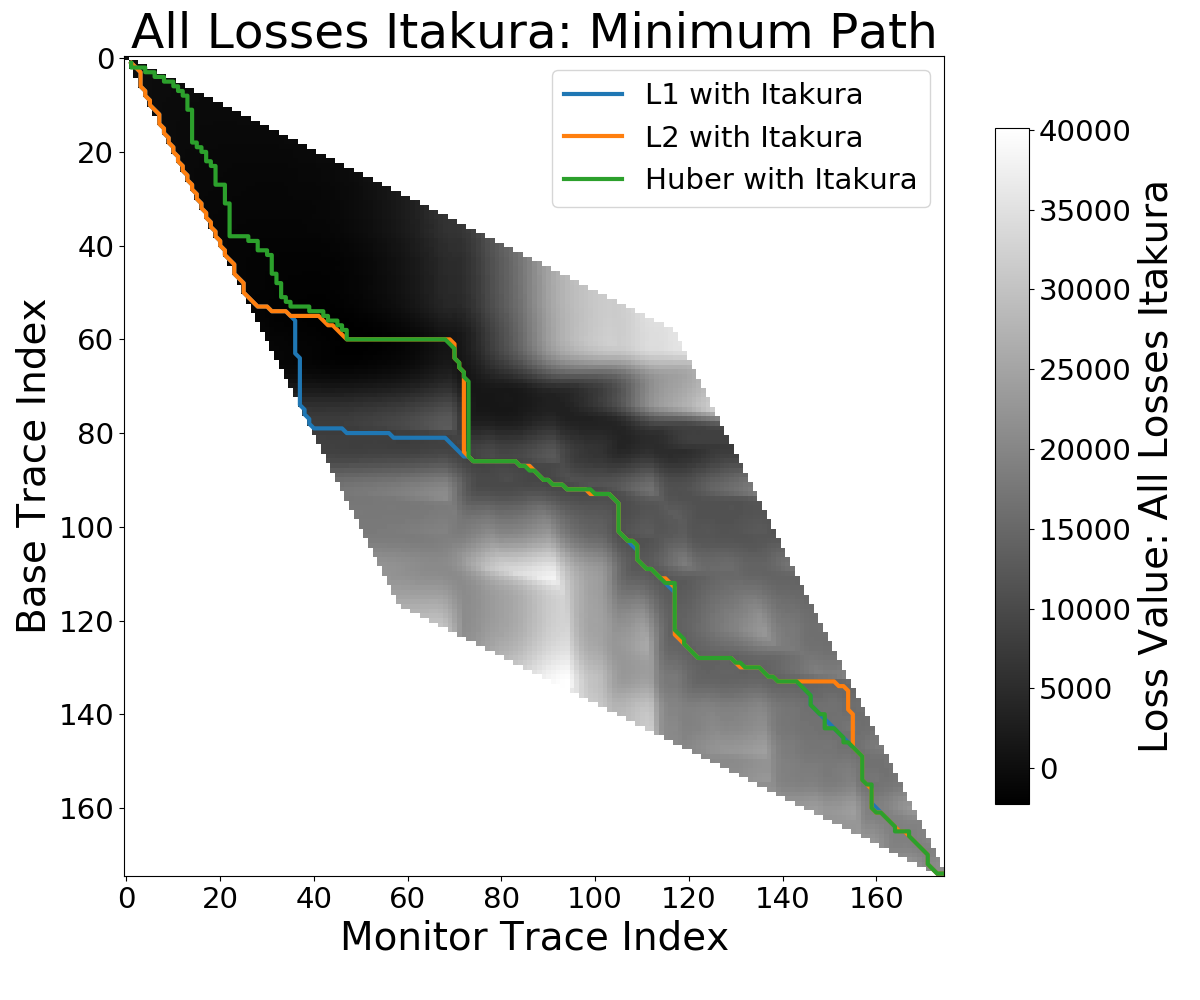
\includegraphics[width=.3\textwidth]{figures/minimum_path_all_losses_itakura_.png} \label{fig:itakura}
    }
    ~
    \subbottom[\citet{Sakoe1978} Disc]{%
     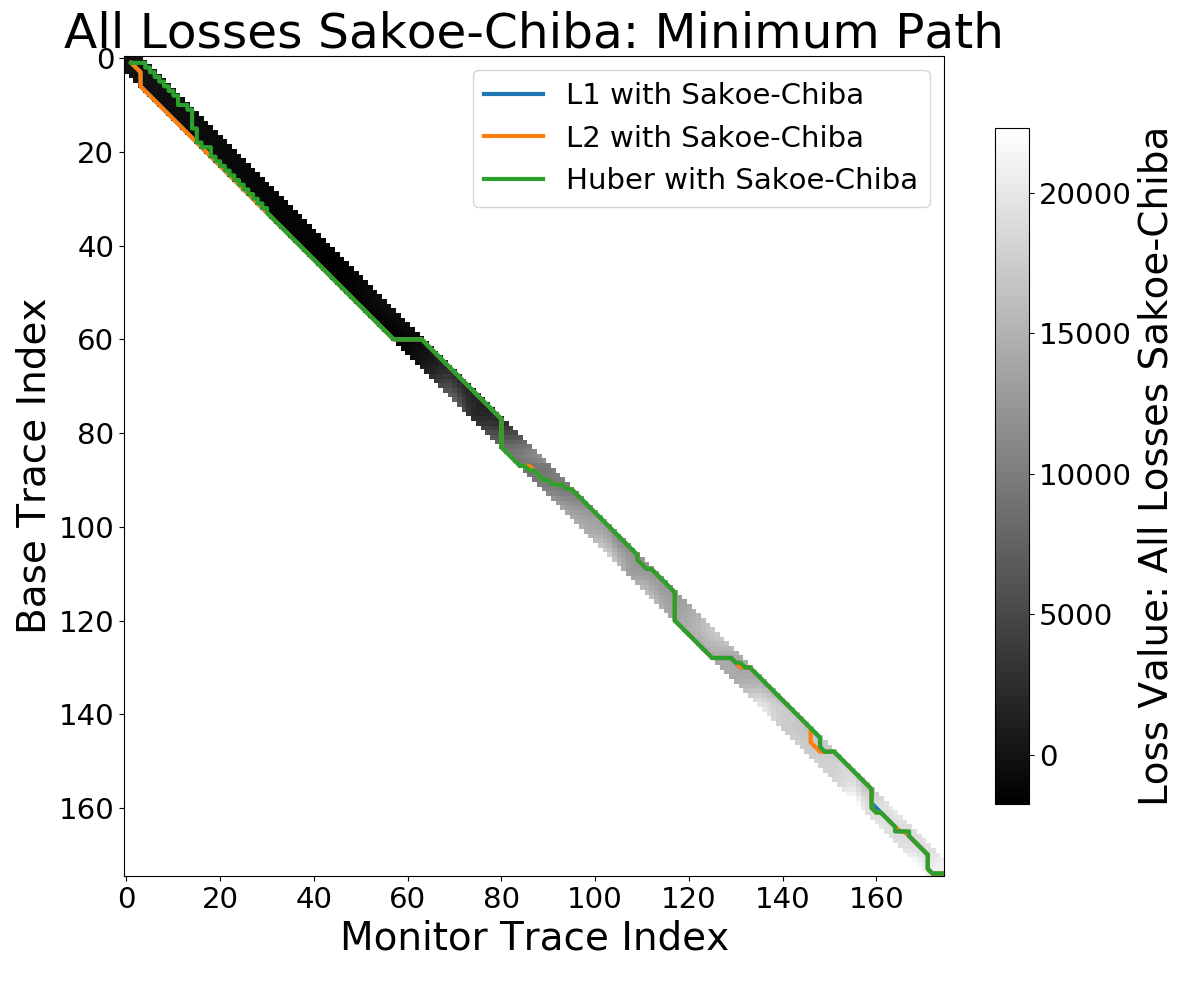
\includegraphics[width=.3\textwidth]{figures/minimum_path_all_losses_sakoe_chiba_.png} \label{fig:sakoe}
    }
    ~
    \subbottom[LB\_Envelope \citep{keogh2005exact}]{%
     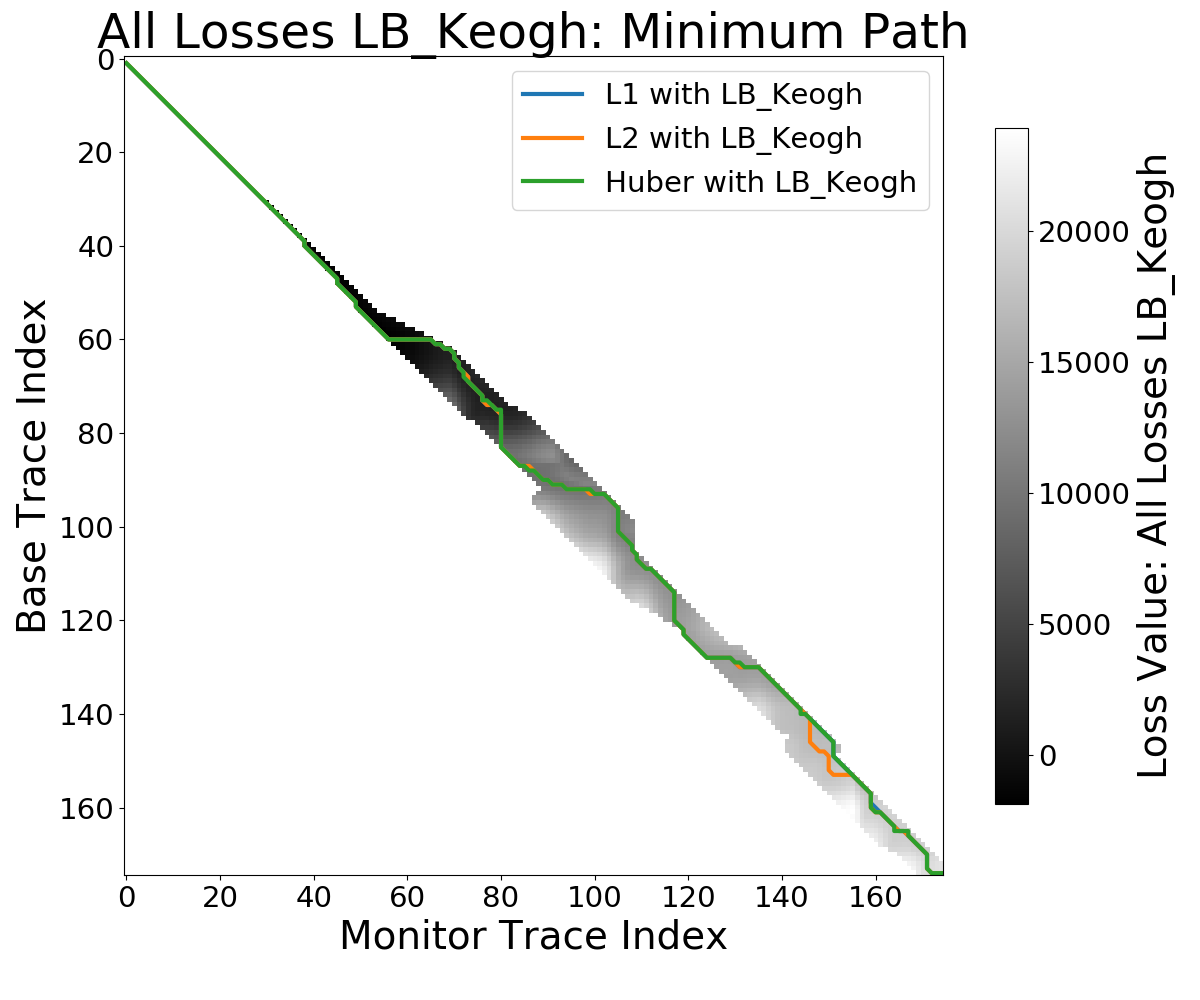
\includegraphics[width=.3\textwidth]{figures/minimum_path_all_losses_lb_keogh_.png}\label{fig:lbk}
    }
\caption{Minimum path for constraint masks for cumulative cost in \ac{dtw}. Images show the optimum path for different loss functions $L_1$, $L_2$, and Huber loss \citep[from][]{dramsch2019dtw}}
\label{fig:constraints}
\end{figure} 
% dramsch2019dtw
\citet{dramsch2019dtw} presents a tutorial of \acf{dtw}. \ac{dtw} is a powerful signal processing tool introduced to 4D seismic analysis by \citep{Hale2013} on synthetic data. 4D seismic data relies on alignment of the seismic volumes. This enables interpreters to compare the amplitudes differences of the data. Due to the capability of \ac{dtw} to match arbitrary time-series, it is applicable to 4D time shifts, seismic-well ties, well-to-well ties, and seismic pre- and post-stack migration \citep{Luo*2014}.  \ac{dtw} is known to be computationally slow and expensive, while extracting poor matches on seismic field data. This tutorial paper goes into detail of the \ac{dtw} algorithm, exploring similarity measures, optimization, and constraints interactively through reproducible implementation in Python.

\begin{algorithm}
\begin{algorithmic}
\Procedure{DTW}{$a,b$}
\State Given: Trace $a$ and Trace $b$ of lengths $n$.
\Function{Calculate distance matrix $D$}{$a,b$}
    \State $D \gets dist(a,b)$
\EndFunction
\Function{Calculate Cumulative Cost $C$}{$D$}
\State $C[0,0] \gets 0$
\For {$i = 1$ to $n$} \Comment{Populate Edge}
    \State $C[0,i] \gets D[0,i] + C[0,i-1]$
    \State $C[i,0] \gets D[i,0] + C[i-1,0]$
\EndFor
\For {$i = 1$ to $n$} \Comment{Fill Cumulative Cost Matrix}
    \For {$j = 1$ to $n$} 
        \State $C_{min} \gets \textbf{min} \{C[i,j-1], C[i-1,j-1], C[i-1,j]\}$
        \State $C[i,j] \gets D[i,j] + C_{min}$
    \EndFor
\EndFor
\EndFunction
\Function{Backtrack minimum cost path $P$}{$C$}
\State $P \gets C[n,n]$
\While {$i > 0 | j > 0$}
    \State $i, j \gets \textbf{index} \{ P[last] \}$
    \State $C_{min} \gets \textbf{min} \{C[i,j-1], C[i-1,j-1], C[i-1,j]\}$
    \State $P.\textbf{append} \gets \textbf{index} \{ C_{min} \}$
\EndWhile
\EndFunction
\State \Return {P}
\EndProcedure
\end{algorithmic}
\caption{\acl{dtw} algorithm consists of calculating the element-wise distance matrix, cumulative cost and then find the optimal path in the cumulative cost matrix} \label{dtw}
\end{algorithm}

The \ac{dtw} algorithm, represented in \cref{dtw}, relies on calculating a distance matrix sample-wise between two traces. This is the first avenue of optimization we explore in this paper. The commonly used $L_1$ norm to calculate the distance norm is shown to perform worst out-of-the-box calculating $|b-a|$. Alternatively, the euclidean distance or $L_2$ norm can be used, which modifies the calculation to $(b-a)^2$. The difference between $L_1$ and $L_2$ is significant in the sense that the $L_1$ norm is not differentiable or convex, however it scales linearly for outliers. The $L_2$ norm converges fast close to zero, however the error "explodes" for outliers. We introduce a constraint used in convex optimization, which combines the advantages of the $L_1$ norm and $L_2$ norm, namely the Huber loss:

\begin{equation}
L_\delta (a, b) = 
\begin{cases}
 \frac{1}{2} (b-a)^2 & \text{for } |b-a| \le \delta, \\
 \delta (|b-a| - \frac{1}{2} \delta), & \text{otherwise.}
\end{cases}
\label{eq:huber}
\end{equation}

which is convex for small values, scales linearly for outliers and is differentiable for all values of $\mathbb{R}$, with $\delta$ being a scaling factor.

Additionally, the search space on the cumulative distance matrix can be constrained to both increase performance and avoid non-optimal solutions. The different contraint strategies are presented in \cref{fig:constraints}. The Itakura parallelogram \citep{Itakura1975} in \cref{fig:itakura} describes a parallelogram that that has the largest width agress the diagonal of the matrix, providing the most flexibility for the \ac{dtw} algorithm in the center parts of the seismic traces. The Sakoe-Chiba disc \citep{Sakoe1978} follows a different strategy, which provides a constant maximum warp path. This strategy in \cref{fig:sakoe} introduces a global maximum time shift. Contrary to these two global constraints, we introduce the LB\_Keogh \citep{keogh2005exact} constraint in the paper. This lower bounding method provides a mathematical lower bound for the \ac{dtw} algorithm. We use this lower bound to constrain the warp path, which provides larger variability to high amplitude areas, where cycle-skipping can occur, presented in \cref{fig:lbk}. The results of combining the Huber loss with the LB\_Keogh constraint are presented in \cref{fig:time-shifts-warped}.

\begin{figure}[!ht]
    \centering
    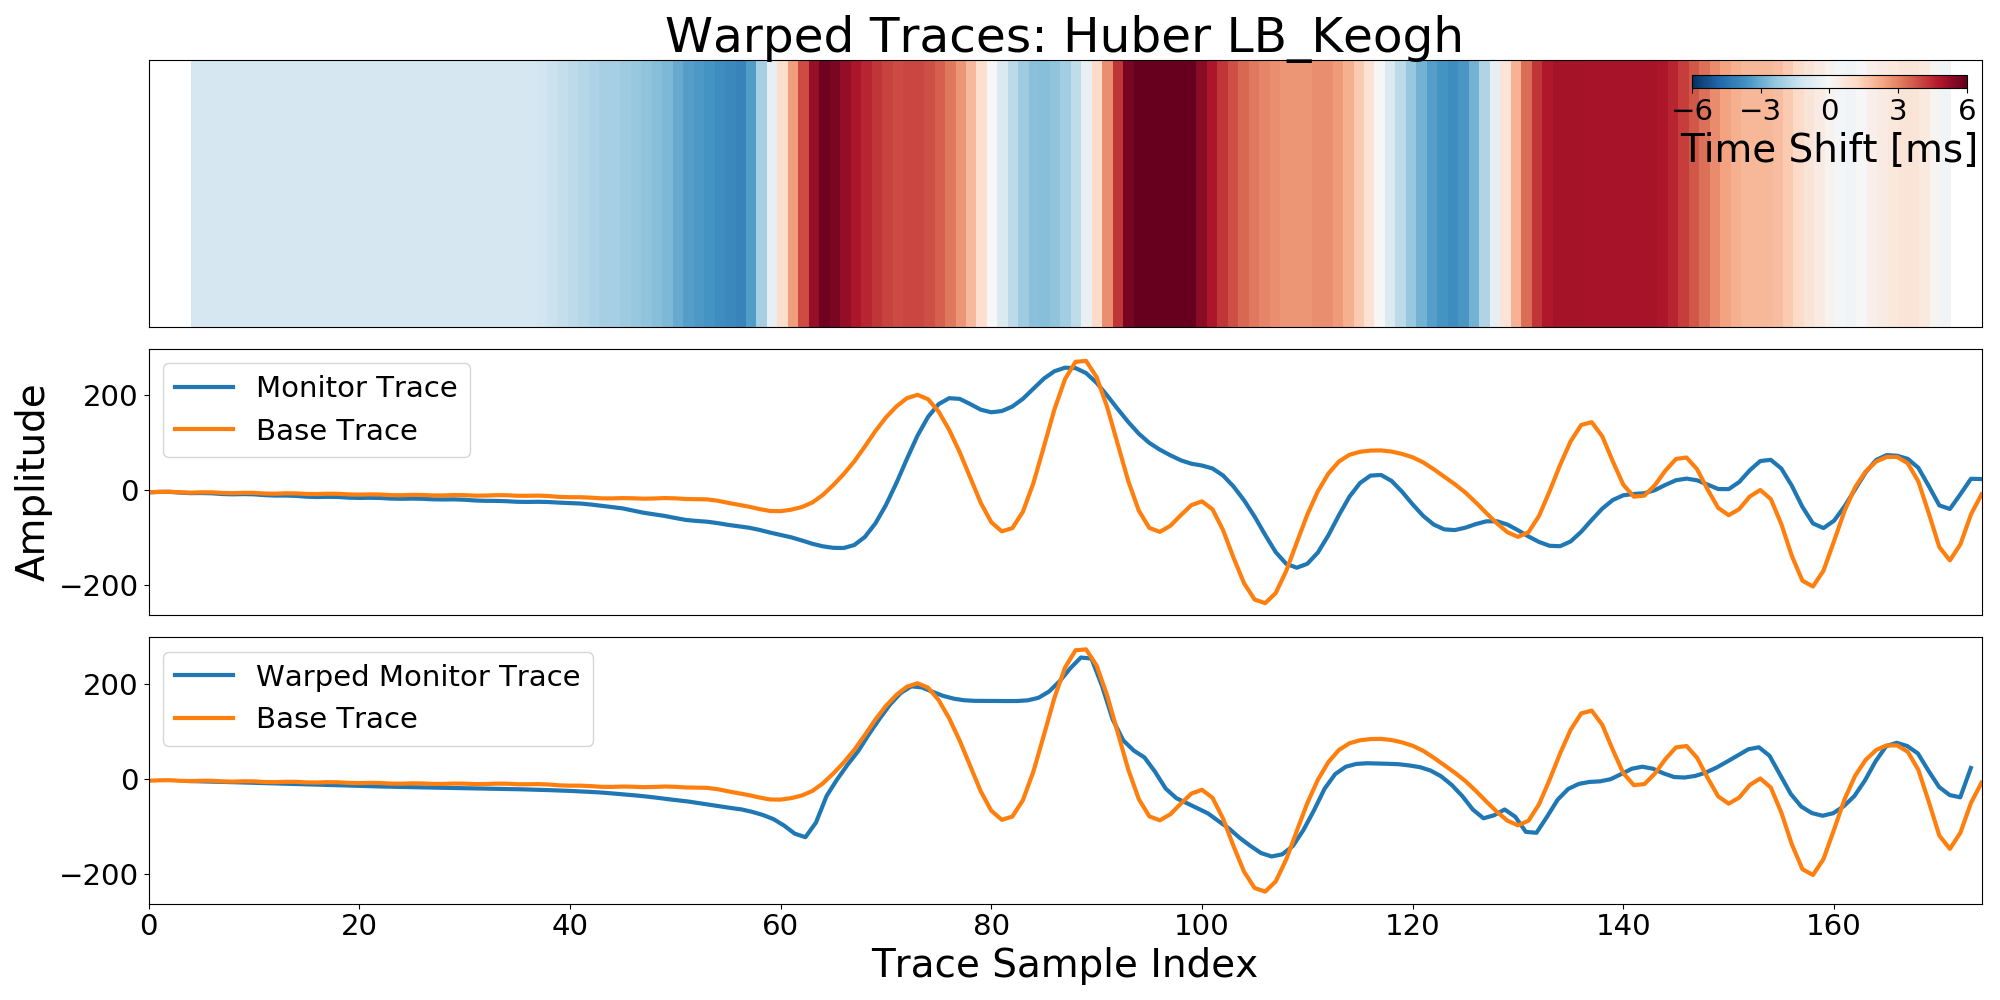
\includegraphics[width=\textwidth]{figures/time_shift_huber_lb_keogh.png}
    \caption{Time shifts and warped traces \citep[from][]{dramsch2019dtw}}
    \label{fig:time-shifts-warped}
\end{figure}

% dramsch2018information
In the workshop paper \citetitle{dramsch2018information} \citep{dramsch2018information} the insight from applying the LB\_Keogh constraint was transferable to \acp{cnn}. \acp{cnn} apply a windowed convolution to the input data. Windowed areas of non-stationary physical data can be offset from the usually baselevel of an amplitude of zero. In the case of seismic data, traces tend to be zero-centered. In the case of a simple activation of a single neuron in a \ac{nn} with $\sigma(w\cdot x + b)$ (cf. \cref{section:nn}), this equates to a bias of $b=0$. Seismic data contains sections that fall within the range of most patches, where the reflection response is entirely offset from zero, which equates to a mean-shift within the network. This paper served as a preliminary study for \citet{dramsch2019complex}, which explores a solution for this property of patch-based training in \acp{cnn} that deteriorates the generalization.

\begin{figure}
    \centering
    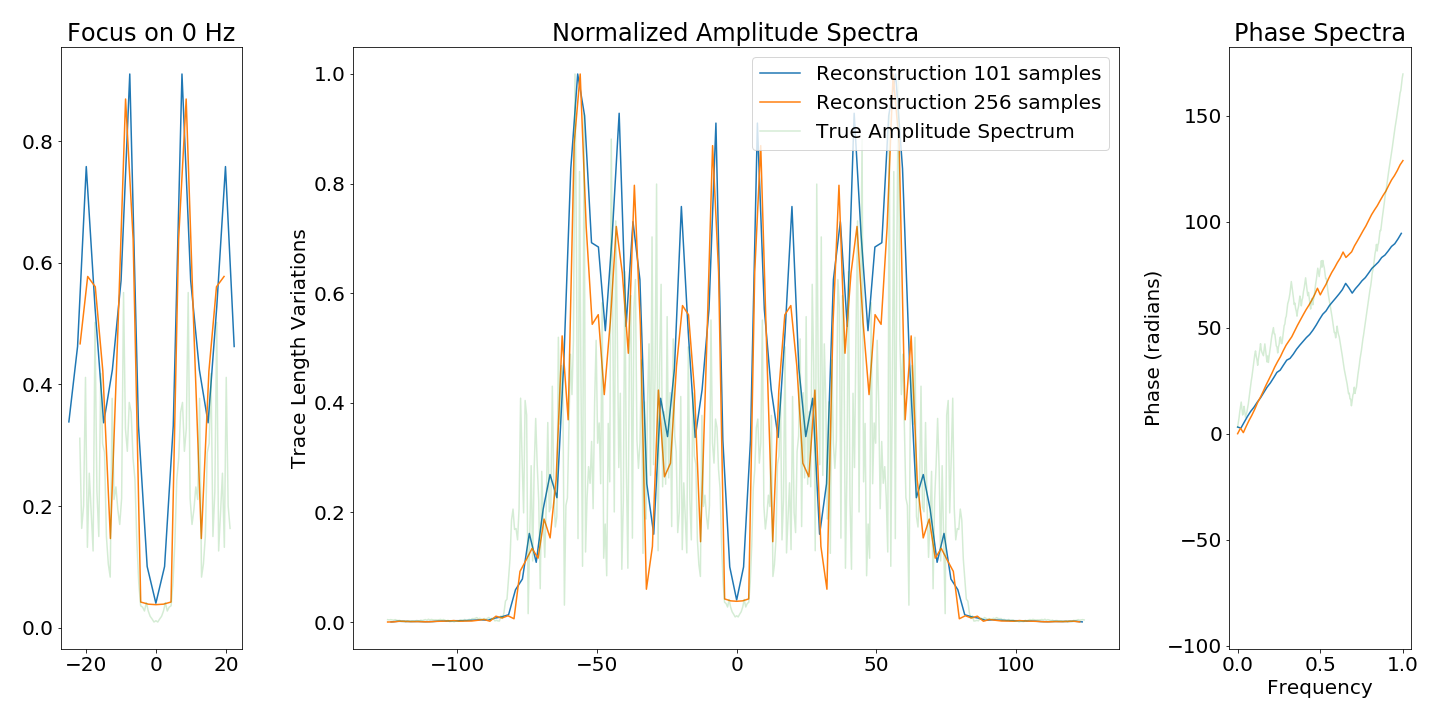
\includegraphics[width=\textwidth]{figures/information-windowing.png}
    \caption{Normalized spectra of windows of trace with "offset" zero. Aliasing of the low frequencies is visible.Phase information not reconstructed from windowed data, slope depending on the window size. Data tapered before \ac{fft} \citep[from][]{dramsch2018information}}
    \label{fig:seismic-window}
\end{figure}

\aclp{nn} apply real-valued transformations on the data, discarding phase information entirely. \cref{fig:seismic-window} shows the spectra of the full trace in green as a background, with two selected cutouts of different sizes overlaid. It is clear that both windows show a sufficiently good reconstruction of the original amplitude spectrum, except for the offset at the low frequencies. The slope of the phase spectrum is reconstructed somewhat by the larger window, but non can reconstruct the notch. Many deterministic signals contain significant information in the phase of the signal. Discarding the phase information leads to low-frequency aliasing analogous to the Nyquist-Shannon theorem for high frequencies.

% dramsch2019complex
In the paper \citetitle{dramsch2019complex} \citep{dramsch2019complex} I explore complex-valued deep convolutional networks to leverage non-linear feature maps and show that in non-stationary data, the phase content improves generalization of \acp{cnn}. Furthermore, complex-valued networks result in a smaller network with better performance compared to a larger real-valued network. In this study I implemented a deep convolutional \acl{ae} to compress 2D slices from a 3D seismic cube to evaluate the reconstruction error. There is a difference of network implementations, where complex-valued neurons are represented as two feature maps, one for the real component and complex component each. Therefore, matching the networks proved to be a complicated task, which led me to build four different architectures that get progressively bigger and compare the results.

The work in \citetitle{dramsch2019complex} \citep{dramsch2019complex} was in part based on reconstruction to test lossy compression and reconstruction of seismic data. Another reason to implement an unsupervised method was the limited availability of realiable interpretations of seismic data. Defining a decision boundary for seismic interpretation is only in the beginning stages of research, which leads us to the decision to inspect reconstructed seismic numerically as signal analysis is well-explored in seismic data processing. Therefore, analysing the result in the \ac{fk}-domain was possible and gave additional insight to the denoising effect of the \ac{ae}.

Nevertheless, some interpretations are available openly and companies often have a plethora of interpretations and re-interpretations of seismic data, making automatic seismic interpretation a topic of interest as evidenced by \cref{tab:geonn}. However, \aclp{dnn} are notorious for needing large numbers of diverse annotated samples. That is often prohibitive to geoscience applications of \acl{ml}. In \citetitle{dramsch2018deep} \citep{dramsch2018deep} we show that \aclp{sota} \aclp{cnn} pre-trained on ImageNet can be transferred to perform \acl{asi}. \cref{fig:asi} shows the results of a fully trained network compared to a pre-trained network. The pre-trained network decreases both training time and data requirements significantly, while not compromising accuracy. A pre-trained network with diverse generalizable learned filters seems to alleviate some limitations of smaller non-diverse data sets used in the fine-tuning process.

\begin{figure}[!ht]
    \subbottom[Waldeland CNN trained from scratch]{%
     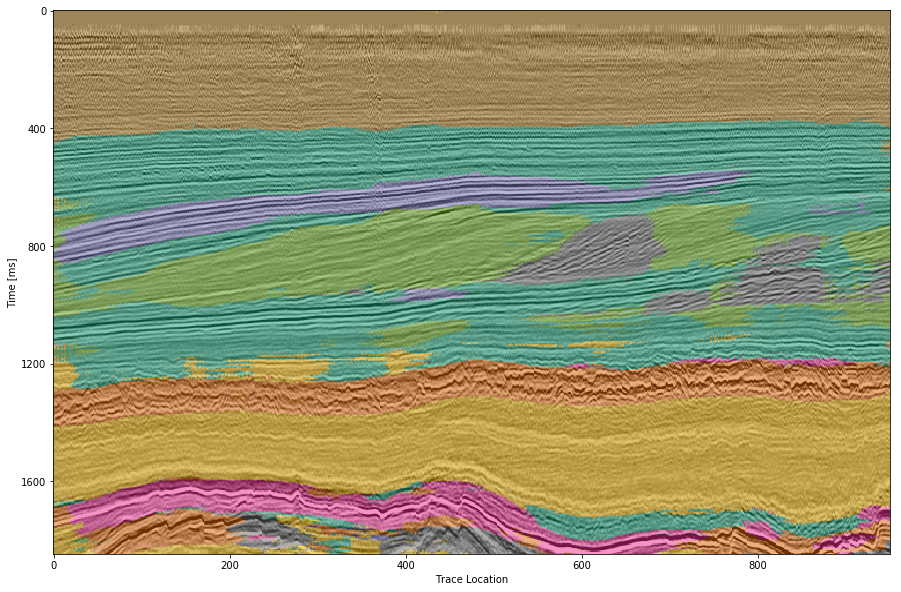
\includegraphics[width=.5\textwidth]{figures/pred1_i.png} \label{fig:asi_pred_waldeland}
    }
    \subbottom[Pre-trained VGG-16]{%
     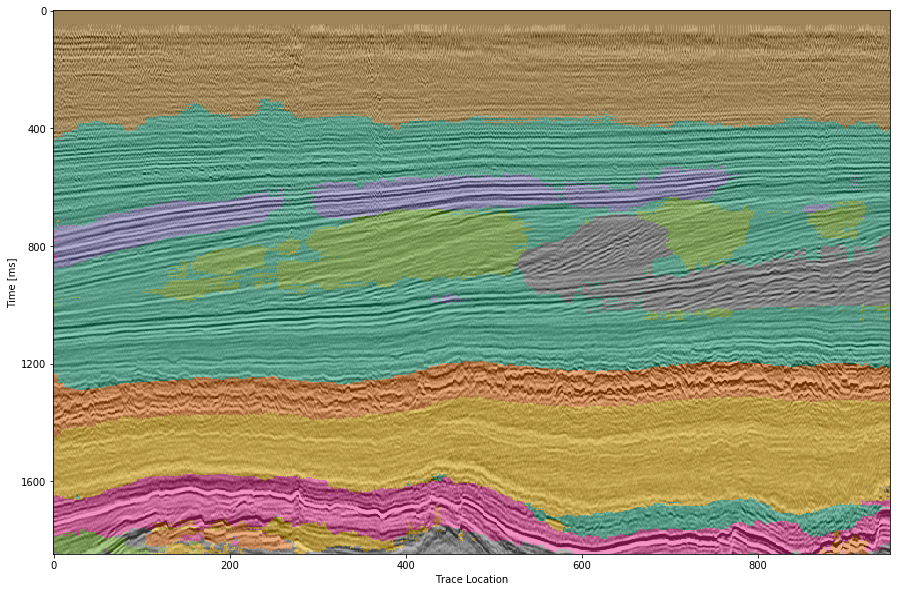
\includegraphics[width=.5\textwidth]{figures/vgg1_i.png} \label{fig:asi_pred_vgg}
    }
\caption{\acl{asi} on two networks, trained from scratch and fine-tuned on pre-trained VGG-16 architecture. The pre-trained network generating a more consistent seismic interpretation, however showing an overall deficiency in diverse training data \citep[from][]{dramsch2018deep}}
\label{fig:asi}
\end{figure}

This chapter summarizes the foundational work conducted to enable the developments of concrete applications of \acl{dl} in geophysics. These foundations touch on signal processing fundamentals in 4D seismic exploring metrics and constraints, then introducing a new constraint for \acl{dtw} in 4D seismics. The work in \aclp{dnn} includes an investigation into aliasing of patch-based training of \aclp{cnn} and including phase information in complex-valued neural networks. Finally, leading to an exploration of transfer learning for efficient training of deep learning models in \acl{asi}.

%!TEX root = ../Thesis.tex
\section{Machine Learning in 4D Seismic Inversion}

A primary application of \acl{ml} is building regression models. These regressions are suited for application in physical inversion problems, considering the value of priors in non-unique solution spaces. This chapter consists of two workshop papers that illuminate a \ac{dl} solution approach from a network architecture analysis in the paper titled \citetitle{dramsch2019including} \citep{dramsch2019including} and a data perspective in the paper titled \citetitle{dramsch2019deep} \citep{dramsch2019deep}.

\begin{figure}
    \centering
    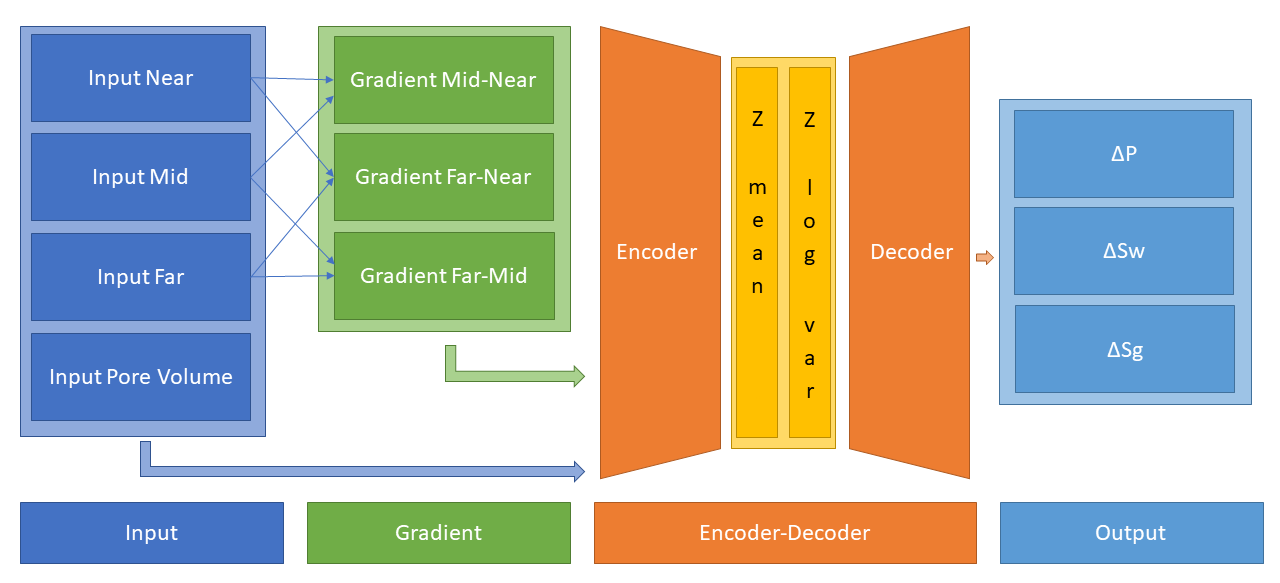
\includegraphics[width=\textwidth]{figures/AVO-Net.png}
    \caption{Architecture includes automatic physics-based gradient calculation of input seismic and an variational encoder-decoder architecture to invert seismic data for pressure and saturation changes \citep[from][]{dramsch2019including}}
    \label{fig:avo-net}
\end{figure}

Traditionally, 4D seismic \acf{qi} often relies on priors to reduce variance in the face of uncertainty. The inversion problem in this chapter is a pressure-saturation inversion from seismic amplitude difference maps in the Schiehallion field. The Schiehallion field is a stacked turbidite reservoir in the UK North Sea, which makes it very heterogeneous and compartmentalized. The T31 sandstone reservoir has the most lateral extent with the thickness ranging from 5~m to 30~m. The small thickness of the reservoir layer results in the entire reservoir being contained in a single trough of a seismic wavelet, which leads us to treat the network as a 2D map instead of a 3D problem. The data available consists of simulation and field data with several timesteps of seismic data in near-, mid-, and far-angle stacks, and pore volumes, as well as, pressure changes and saturation changes for water and gas from simulation.

In \citet{dramsch2019including} we present a novel network structure that explicitly includes AVO gradient calculation within the network as physical knowledge, shown in \cref{fig:avo-net}. The network architecture was chosen to follow an encoder-decoder architecture as a forcing function for information distillation. Additionally, the bottleneck layer implements a variational encoding layer to be less susceptible to noisy input. The network explicitly includes AVO gradient calculation in the network architecture, considering it is physical knowledge we know will stabilize pressure and saturation change separation. Including basic physics knowledge leads to the network learning residual information, essentially defining another forcing function for the networks learning process.

The initial phase was carried out on simulation data with a train test split, leaving a full 4D time step as validation set. \acl{nas} was applied to the network to determine depth and width of the architecture, using a \ac{tpe} hyper-parameter search \citep{bergstra2015hyperopt}. Afterwards, to transfer the network to field data, the input of the network was combined with additive Gaussian noise \citep{bishop1995training} to train the network for noisy field data input. This was a manual process of estimating good noise levels.
%\aclp{dnn} can learn these data-dependent priors from training data.

\begin{figure}
    \centering
    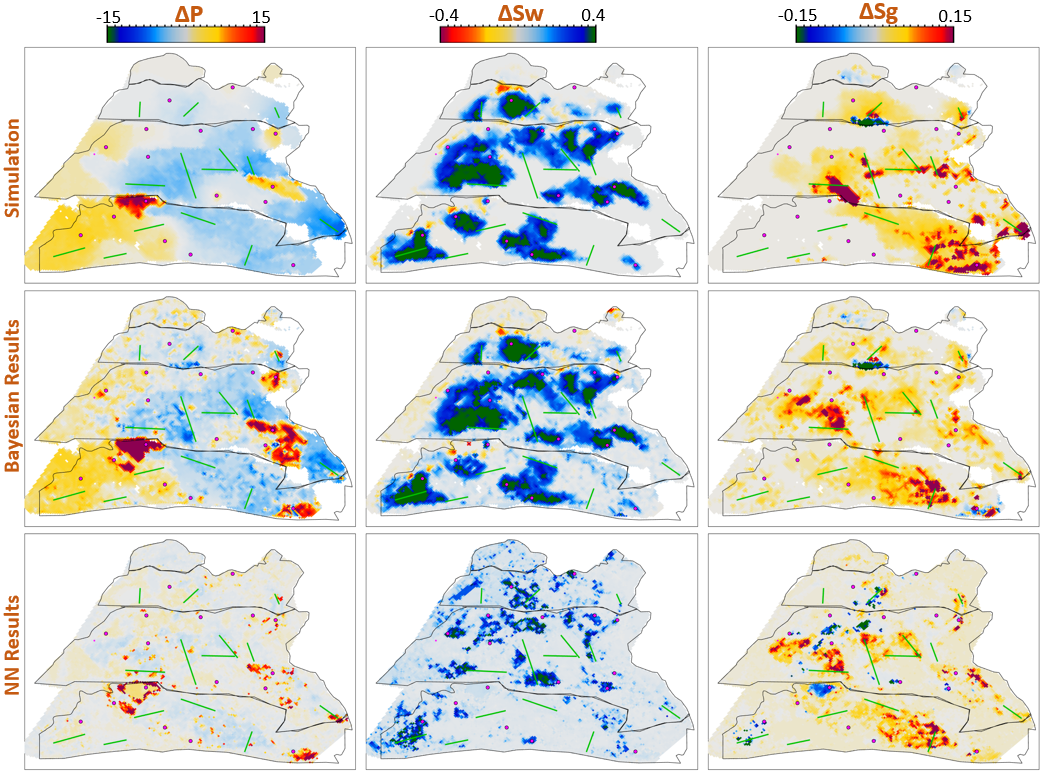
\includegraphics[width=\textwidth]{figures/NN_results.PNG}
    \caption{4D QI inversion results from Bayesian inversion and \acl{nn} inversion. Bayesian inversion closely resembles simulation output. \ac{nn} result showing good coherency, consistent amplitudes, but problems in strong changes of gas saturation \citep[from][]{dramsch2019deep}}
    \label{fig:avo-net-results}
\end{figure}

The workshop paper \citet{dramsch2019deep} contains these results compared to the simulation results and Bayesian inversion results, shown in \cref{fig:avo-net-results}. These initial results on limited training data show that the stochastic process can extract pressure saturation information from field data, after training on simulation data. While the overall result is promising, regions of strong gas saturation changes present a problem. This could be contingent problems in the modelling as well as the fact, that they generate strong amplitude differences and are far in between, essentially behaving like outliers. 

Learning meaningful information in deep neural networks is often contingent on interpreting the neural network. The results presented in \cref{fig:avo-net-results} contain three indicators that the network learned a meaningful inversion regression for the Schiehallion field. The network gets the overall trend in increase and decrease of pressure and saturation correct. Additionally, the range of output values for the network is unconstrained, but the network provides values in the ranges, that are expected from the simulation and Bayesian inversion results.  However, and more interestingly, the networks does not contain spatial information, being a feed-worward \ac{dnn} not a \ac{cnn}, yet returns continuous albeit noisy outputs when assembled into maps.

This chapter comprised of two workshop papers, shows a working implementation of a machine learning system inverting pressure-saturation data from seismic. Moreover, an implementation of a network trained on simulation data that is transferred to field data by noise modelling is presented. Finally, we show that including basic physics in the network architecture stabilizes training, making the case for physics-based \acl{ml}. Two journal papers are in preparation but not included in this thesis that analyze the network structure and the training data in detail \citep{corte2019exploring,dramsch2020physics}. 


% dramsch2019physics
% We present a novel neural network architecture that trains on synthetic data and provides insights into observed field seismic. The network explicitly includes AVO gradient calculation within the network as physical knowledge to stabilize pressure and saturation changes separation. We apply the method to Schiehallion field data and go on to compare the results to Bayesian inversion results. Despite not using convolutional neural networks for spatial information, we produce maps with good signal to noise ratio and coherency.

% dramsch2019deep
% Geoscience data often have to rely on strong priors in the face of uncertainty. Additionally, we often try to detect or model anomalous sparse data that can appear as an outlier in machine learning models. These are classic examples of imbalanced learning. Approaching these problems can benefit from including prior information from physics models or transforming data to a beneficial domain. We show an example of including physical information in the architecture of a neural network as prior information. We go on to present noise injection at training time to successfully transfer the network from synthetic data to field data.

%!TEX root = ../Thesis.tex
\section{Machine Learning in 4D Seismic Time-Shift Extraction}

This final chapter consists of the submitted journal paper \citetitle{dramsch20193dwarping} \citep{dramsch20193dwarping}. This paper presents a novel 3D warping technique for the estimation of 4D seismic time-shifts. The algorithm is unsupervised and provides 3D warp-fields with uncertainty measures, while avoiding many limiting assumptions.

4D seismic time shift extraction is often done in 1D, due to time constraints and often sub-par performance of 3D algorithms. This chapter explores and summarizes conventional 3D warping methods and machine learning approaches. Many of these algorithms rely on classical cross-correlational or optical flow approaches. Correlation-based algorithms can be susceptible to noise and inversion-based algorithms can take weeks to provide results and optical flow approaches suffer from the implicit assumption in standard implementations. These approaches suffer from the same limitations in \acl{ml} systems just like conventional algorithms. In this chapter the medical Voxelmorph algorithm is adapted to match 4D seismic data volumes in 3D.

The Voxelmorph algorithm is based on the diffeomorphic assumption, which at its core describes the map of one data set to another data set, providing this map with particular properties. The main benefit of applying diffeomorphic mapping to geoscience data comes in the fact that all diffeomorphisms are homeomorphic. The homeomorphic assumption transfers well to the geological reality that the mathematical topology stays constant, resulting in reflectors neither crossing nor generating loops. 

The algorithm is trained in an unsupervised, or rather self-supervised way to avoid the bias from time shifts that were extracted from any other method. Supervised training is discussed in the paper as implicitly introducing the assumption of the extraction method for the training data into the newly trained network.

\begin{figure}
    \centering
    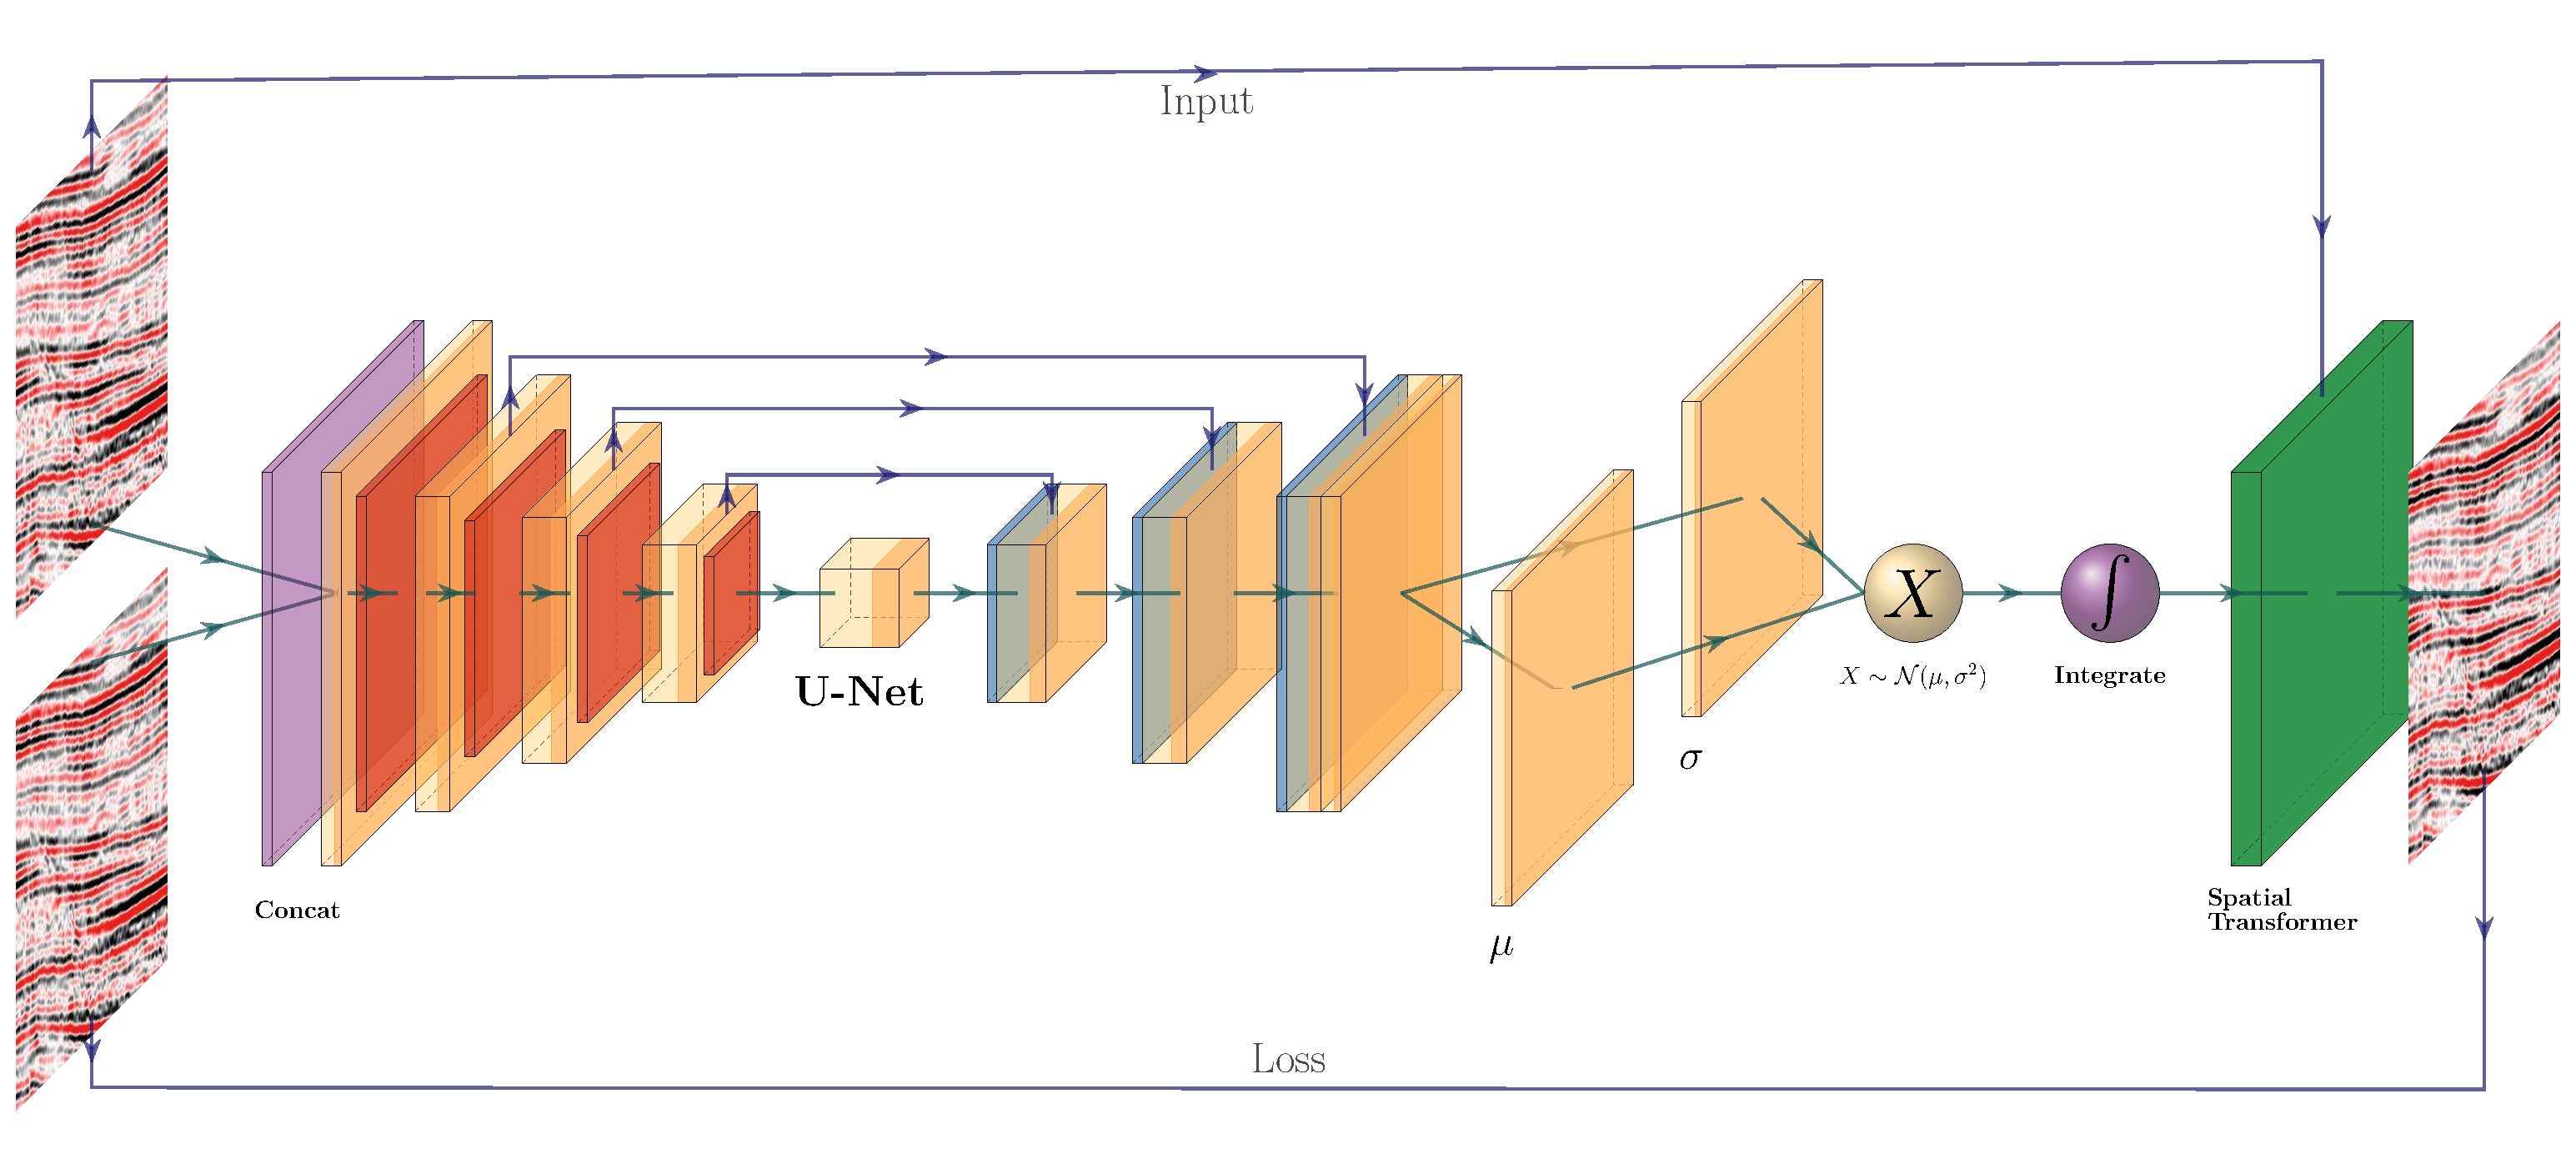
\includegraphics[width=\textwidth]{figures/Voxelmorph.pdf}
    \caption{Voxelmorph Architecture 2D abstraction. Two 3D volumes are passed to the network, concatenated (purple) and passed to a U-Net architecture. The U-Net outputs two cubes that generate the mean static velocity and the standard deviation, which is sampled during training. The sampled value is integrated to obtain the diffeomorphic warp velocity used in the spatial transformer layer (green). The network evaluates losses on the \ac{kl}-divergence at $\mu, \sigma$ and \ac{mse} between the warp result of the monitor volume and the warped base volume, enabling self-supervised training \citep[from][]{dramsch20193dwarping}}
    \label{fig:voxelmorph}
\end{figure}

The architecture in the network uses the U-Net architecture to input two 3D seismic volumes and extract a static warp velocity field, shown in \cref{fig:voxelmorph}. The static velocity field is extracted as a Gaussian distribution to measure the co-variance and provide uncertainty value of the three-dimensional warp field. The neural network itself does not warp the seismic data, to increase transparency of the process. The architecture following the U-net samples the extracted velocity distribution and integrates this value to obtain the diffeomorphic flow. These values are passed to a dense 3D warping mechanism to enable the unsupervised training. The losses involved are a \acf{kl}-divergence on the stationary velocity field and \ac{mse} on the difference between that warped monitor volume and the base volume.

In the paper we present the modified self-supervised \acl{nn} system and test the results on the training data itself and two generalization test sets. The first test set is on the same field but recorded at different times to the training set, ensuring a similar underlying geology, whereas, the second test set is taken from an adjacent field, recorded at different times, testing the full transfer of the trained network. We go on to test the original Voxelmorph architecture, which uses upsampled velocity fields and evaluate the results against our modified architecture, which uses the full flow field. Overall, this technique introduces a generalizable \acl{dl} approach to extract 3D time-shifts with uncertainty measures from raw stacked 4D seismic data.

\section{Contributions of this Study}

This thesis contributes tangible \acl{ml} applications in geoscience that solve real-world problems as well as work that contributes to the fundamental understanding of signal processing and \aclp{nn} in non-stationary physics.

The explorational work of this thesis validates the impact of image processing for enhancing the resolution of seismic data and automatic fault extraction. This work bridged the scale-gap between local \acl{bhi} and regional seismic data. The exploration of \acl{bsem} data introduced a novel unsupervised method to extract chalk grain boundaries from image data and shows the improvement of subsequent morphological filtering. These methods reduce labor-intensive manual tasks, introducing varying degrees of automation in geoscience workflows.

The foundational work investigates low-frequency aliasing in \aclp{cnn} and goes on to show that phase information in complex-valued neural network can stabilize the reconstruction of compressed seismic data. The smaller complex-valued network outperforms larger real-valued networks, however, a very large real-valued network can implicitly learn partial phase information \citep{dramsch2019complex}. The paper touches on deficits of current metrics applied to geoscience and exposes a periodic dimming effect of frequencies from neural networks that should be further investigated, particularly in the context of aliasing. This paper led to the creation of the open source software package \texttt{keras complex} to enable complex-valued deep learning in \texttt{\acl{tf}} (Manual in \ref{section:keras-complex}). The code was available in an older framework \citep{trabelsi2017deep}, which I consolidated for this study. I went on to package the code, make it easily installable and generate online documentation to enable researchers to generate their own studies from this work \citep{dramsch2019complexcode}.

The research in \citet{dramsch2018deep} showed that transfer learning can alleviate the necessity for large amounts of labeled data, by re-using a neural network on natural images. This study showed the generalizable networks can be transferred to seismic data and outperform smaller networks trained from scratch, the smaller network size being necessary to avoid overfitting. The source code for this research was made available and has been re-used multiple times \citep{dramsch2018deepcode}. This has wide applications in industry and research settings, considering the limited availability of labeled data and wide availability of pre-trained network architectures. Moreover, this insight is applicable to pre-training geoscientific \aclp{nn} and fine-tuning these models to specific applications when needed.

The tutorial paper \citep{dramsch2019dtw} contributes insights into applications of \acl{dtw} in 4D seismic. This work explores the influence of varying metrics in geoscience, introducing the Huber loss as a possible loss function for geoscientific application. The study goes on to show that a novel application of the LB\_Keogh lower bound for \acl{dtw} can significantly improve the accuracy for field data, introducing a constraint on the search space for \ac{dtw}. The code for this tutorial including further interactive explorations into constraints for \acl{dtw} will be made available after the double-blind peer review process concludes \citep{dramsch2020dtwcode}.

The first application of \acl{ml} to 4D seismic data introduces a novel method to perform pressure-saturation inversion on amplitude difference maps \citep{dramsch2019deep}. This work introduces basic physics principles into the neural network architecture, which was shown to stabilize the training result. Moreover, this work shows the possibility of training \aclp{dnn} on simulation data and subsequently transferring the network to field data, by applying adequate noise injection. The \acl{dnn} results were successfully compared to results from the Bayesian inversion showing a promising application of \aclp{dnn} in 4D \acl{qi} \citep{dramsch2019deep}. While this work has attracted interest in a sponsors meeting and the workshop presentations \citep{dramsch2019deep,dramsch2019including}, further investigation into model explainability and lower complexity baseline models is necessary \citep[in preparation][]{corte2019exploring,dramsch2020physics}.

The second application of \acl{ml} to 4D seismic data presents a completely novel method for time-shift extraction \citep{dramsch20193dwarping}. This method combines recent advancements in diffeomorphic mapping, \acl{dl} and unsupervised learning to introduce a 3D time shift extraction method including uncertainty values, where 1D extraction is the standard. The method is shown to work on 3D seismic post-stack data with strongly differing acquisition parameters, without supplying any time shift information. After applying the method, the 3D seismic volumes are aligned well, with the diffeomorphic constraint performing well on seismic data. The time shifts show that the main variation of the data is along the time axis (z), with minor shifts along x and y close to faults, compensating for illumination differences. This work tests the trained network on two other 3D seismic volume pairs to test the generalization of the \ac{cnn} after training. The two test sets show that the trained model on a single 3D seismic volume pair transfers well to the same field with different acquisition parameters and even a different field with vastly different geological setting. The code is openly available to foster further development and investigation of the method \citep{dramsch20203dwarpingcode}.

Overall, this thesis shows the impact \acl{dl} can have in geoscience with two novel methods for 4D seismic analysis. It shows the impact of fundamental research of signal processing and information theory in \aclp{dnn} and \aclp{cnn}. Moreover, it shows applications of building systems in label sparse environments to leverage technological advancements and the value of including prior physical insights into \acl{ml} workflows. This thesis builds heavily on open source software and aims to return some of effort.